%%%%%%%%%%%%%%%%%%%%%%%%%%%%%%%%%%%%%%%%%
% Short Sectioned Assignment
% LaTeX Template
% Version 1.0 (5/5/12)
%
% This template has been downloaded from:
% http://www.LaTeXTemplates.com
%
% Original author:
% Frits Wenneker (http://www.howtotex.com)
%
% License:
% CC BY-NC-SA 3.0 (http://creativecommons.org/licenses/by-nc-sa/3.0/)
%
%%%%%%%%%%%%%%%%%%%%%%%%%%%%%%%%%%%%%%%%%

%----------------------------------------------------------------------------------------
%	PACKAGES AND OTHER DOCUMENT CONFIGURATIONS
%----------------------------------------------------------------------------------------

\documentclass[paper=a4, fontsize=10pt]{scrartcl} % A4 paper and 11pt font size

\usepackage[T1]{fontenc} % Use 8-bit encoding that has 256 glyphs
\usepackage{fourier} % Use the Adobe Utopia font for the document - comment 
% this line to return to the LaTeX default
\usepackage[english]{babel} % English language/hyphenation
\usepackage{amsmath}
\usepackage{amssymb} % Math packages
\usepackage{graphicx}
\usepackage{listings}
\usepackage{caption}
\usepackage{subcaption}
\usepackage{mathpartir}

%\usepackage{stmaryrd}
%\usepackage{mathrsfs}

\usepackage{lipsum} % Used for inserting dummy 'Lorem ipsum' text into the 
% template

\usepackage{sectsty} % Allows customizing section commands
\allsectionsfont{\centering \normalfont\scshape} % Make all sections centered, 
% the default font and small caps

\usepackage{fancyhdr} % Custom headers and footers
\pagestyle{fancyplain} % Makes all pages in the document conform to the custom 
% headers and footers
\fancyhead{} % No page header - if you want one, create it in the same way as 
% the footers below
\fancyfoot[L]{} % Empty left footer
\fancyfoot[C]{} % Empty center footer
\fancyfoot[R]{\thepage} % Page numbering for right footer
\renewcommand{\headrulewidth}{0pt} % Remove header underlines
\renewcommand{\footrulewidth}{0pt} % Remove footer underlines
\setlength{\headheight}{13.6pt} % Customize the height of the header

% \numberwithin{equation}{section} % Number equations within sections (i.e.  
% 1.1, 1.2, 2.1, 2.2 instead of 1, 2, 3, 4)
% \numberwithin{figure}{section} % Number figures within sections (i.e. 1.1, 
% 1.2, 2.1, 2.2 instead of 1, 2, 3, 4)
% \numberwithin{table}{section} % Number tables within sections (i.e. 1.1, 1.2, 
% 2.1, 2.2 instead of 1, 2, 3, 4)

% \setlength\parindent{0pt} % Removes all indentation from paragraphs - comment 
% this line for an assignment with lots of text

%----------------------------------------------------------------------------------------
%	TITLE SECTION
%----------------------------------------------------------------------------------------

\newcommand{\horrule}[1]{\rule{\linewidth}{#1}} % Create horizontal rule 
 %command with 1 argument of height

\title{	\normalfont \normalsize 
%\textsc{university, school or department name} \\ [25pt] % Your university, 
%school and/or department name(s)
\horrule{0.5pt} \\[0.4cm] % Thin top horizontal rule
\huge Timing Insensitive Noninterference\\ % The assignment title
\horrule{2pt} \\[0.5cm] % Thick bottom horizontal rule
}

\author{Andrew Ferraiuolo} % Your name

\date{\normalsize\today} % Today's date or a custom date
\parskip = 2\baselineskip
\usepackage[parfill]{parskip}
\begin{document}

\maketitle % Print the title

%----------------------------------------------------------------------------------------
%	PROBLEM 1
%----------------------------------------------------------------------------------------

\section{Introduction}

The type system of SecVerilog verifies that a hardware description respects a 
timing sensitive notion of the noninterference property. When the system of 
interest is properly labeled, this can efficiently verify that a system is free 
of undesired explicit, implicit, and timing channels. However, many commercial 
systems are developed with threat models that are not concerned with timing 
channels. For these systems, timing sensitive noninterference may be overly 
restrictive, causing many reasonable designs to be rejected and forcing 
unnecessary and costly changes to the hardware. In this document we illustrate 
the limitations of timing sensitive noninterference in SecVerilog. We then show 
how a timing insensitive formulation of noninterference familiar to the 
software domain can be beneficially applied here. Finally, this document shows 
that timing sensitivity is free and compulsory in hardware and contrasts this 
with software timing sensitivity.

\section{Timing Sensitivity and Restrictions}
The security policy of SecVerilog, an inherently concurrent HDL, is based off 
of Observational Determinism, a noninterference policy variation that addresses 
concurrency. The policy used in SecVerilog is altered slightly to account for 
dependent labels which allow the security level of a variable to change. The 
authors define a low-equivalence relation $\approx_l$ on states $\sigma$ for a 
given level $l\in \mathcal{L}$ by
\begin{align*}
    \forall \sigma_1, \sigma_2. \sigma_1 & \approx_l \sigma_2 
    \Longleftrightarrow \forall x \in Vars \\
        & (\mathcal{T}(x,\sigma_1) \sqsubseteq l
        \Leftrightarrow \mathcal{T}(x,\sigma_2) \sqsubseteq l) \\
        \wedge & ( \mathcal{T}(x,\sigma_1) \sqsubseteq l \Rightarrow
        \sigma_1(x) = \sigma_2(x) )
\end{align*}
where $\mathcal{T}(x, \sigma)$ denotes the value of $\Gamma(x)$, the type 
environment, in state $\sigma$. Note that the first part of the conjunction 
prevents leakage through observable changes in dependent types.

The authors then define observational determinism as a property of traces $T$ 
which are sequences of events $(t,\sigma)$ where $t$ is a clock cycle. They 
write $\langle \sigma, Prog\rangle \hookrightarrow T$ when program $Prog$ can 
produce trace $T$ in initial state $\sigma$. Note that a program can produce 
multiple traces. Observational determinism of program $Prog$ holds if for any 
$\sigma_1$ and $\sigma_2$
\begin{align}
    \sigma_1 \approx_L \sigma_2 \wedge \langle\sigma_1,Prog\rangle 
    \hookrightarrow T_1
    \wedge \langle\sigma_2,Prog\rangle \hookrightarrow T_2 \\
    \Longrightarrow T_1 \approx_L T_2
\end{align}
where traces are low-equivalent if the states at each cycle are low-equivalent.
The timing sensitivity of SecVerilog can be observed here. Since this condition 
demands cycle-by-cycle equivalence on all traces produced by the program in two 
different states, any timing variation caused by the attacker-unobservable 
portion of the program is deemed insecure.

\begin{figure}
    \begin{center}
        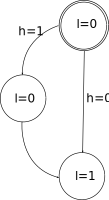
\includegraphics[width=1.2in]{fsm1.pdf}
        \caption{An FSM with a Timing Channel}
        \label{fig:fsm1}
    \end{center}
\end{figure}

The restrictiveness of timing sensitivity at the hardware level can be 
illustrated with the simple FSM of Figure 1 where l is attacker-observable, but 
h is not. Consider low-equivalent initial states $\sigma_1=\{(h,0),(l,0)\}$ and
$\sigma_2=\{(h,1),(l,0)\}$. This FSM is deterministic, so it produces one trace 
in each state,
\begin{align*}
\langle Prog, \sigma_1 \rangle &\hookrightarrow
(1, \sigma_1), (2, \sigma_1[l\mapsto1]) \\
\langle Prog, \sigma_2 \rangle &\hookrightarrow
(1, \sigma_2), (2, \sigma_2), (3, \sigma_2[l\mapsto1])
\end{align*}
Clearly, these traces are not low-equivalent since at cycle 2 $\sigma_1$ 
transitions to a state where l is 1, but $\sigma_2$ does not. However, if we 
assume clock transitions are fast and measurements by the attacker are not 
precise enough to distinguish events on a per-cycle basis, this appears overly 
restrictive. To such an attacker it appears as though in both cases the system 
instantly proceeds to a state with $l=1$.

\begin{lstlisting}[frame=single,caption=An Arbiter in Verilog.]
always @(state, req_1, req_2) begin
  case(state)
    0: next_state <= req_1 ? 1 :
                     req_2 ? 2 :
                     0;
    1: next_state <= req_2 ? 2 : 0;
    2: next_state <= req_1 ? 1 : 0;
    default: next_state <= 0;
  endcase
end

assign grant_1 = (state == 1);
assign grant_2 = (state == 2);
\end{lstlisting}

As a more practical example, Listing 1 shows a verilog code segment for an 
arbiter that grants requests for a high confidentiality module and a low 
confidentiality module. Whether or not the high confidentiality module has a 
request is considered a secret.
The typing environment is
$\Gamma = \tt{\{(state, h), (req_1, h), (grant_1, h), (req_2, l), (grant_2, 
l)\}}$.
Whether or not there is a request on $req_1$ can affect \emph{when} there is a 
grant in response to $req_2$, but since this arbiter prevents starvation, there 
will always be a response either way. As one would expect, this module produces 
unequal traces because of a timing channel. Consider initial states
$\sigma_1 = \{(\tt{req_1}, 1), (\tt{req_2}, 1), (\tt{state}, 0), \dots\}$ and
$\sigma_2 = \{(\tt{req_1}, 0), (\tt{req_2}, 1), (\tt{state}, 0), \dots\}$ 
(where the grants have the appropriate values). Assuming the inputs do not 
change, with each of these states the program generates the traces
\begin{align*}
  \langle Prog, \sigma_1 \rangle & \hookrightarrow
  \tt
    (1, \sigma_1), (2, \sigma_1[state\mapsto1][grant_1\mapsto1),
    (3, \sigma_1[state\mapsto2][grant_2\mapsto1]), (4, \sigma_1) \\
    \tt
  \langle Prog, \sigma_2 \rangle & \hookrightarrow
    (1, \sigma_2), (2, \sigma_1[state\mapsto2][grant_2\mapsto1),
    (3, \sigma_2)
\end{align*}
which are unequal. However, with both initial states $grant_2$ is eventually
$1$ after the request is issued, so this just a timing channel.

\section{Timing Insensitivity with High-Stutter Equivalence}
In ``Enforcing Robust Declassification and Qualified Robustness'' Myers et. al. propose a formulation
of noninterference that does not consider 
timing channels by comparing the $l$-projection of traces. Essentially, the 
$l$-projection of a trace is constructed from a trace by first producing the 
sequence of only the $l$ or lower parts of the states. Then, for any adjacent 
pair of low-equivalent states, all but the first is dropped. The end result is 
a sequence expressing just the states that appear different to the attacker 
ordered chronologically.  

Two traces are said to be high-stutter equivalent if their $l$-projections are 
equal. The formulation of noninterference in Equation 1 can be made timing 
insensitive by replacing the clockwise relation $\approx_l$ on traces with 
high-stutter equivalence. Re-examining the FSM of Figure 1, the $l$-projections 
of the traces $T_1$ and $T_2$ produced by initial states $\sigma_1$ and 
$\sigma_2$ respectively are both $\{(l,0)\}, \{(l,1)\}$, so these traces are 
high-stutter equivalent and the FSM obeys the new formulation of 
noninterference. Similarly, the traces given for the code segment in Listing 1 
both have the $l$-projection
$$
\tt
\{(req_2,1),(grant_2,0)\}, \{(req_2,1),(grant_2,1)\}, \{(req_2,1),(grant_2,0)\}
$$
and so this arbiter appears safe as well.

\section{Enforcement}
A great deal of work has been done on addressing timing channels in software 
languages. These software timing sensitive noninterference systems require 
extensions to a standard (timing insensitive) noninterference type system e.g. 
by code transformation or by labeling the program counter. However, 
noninterference at the hardware level enforces timing sensitivity for free. The 
crucial difference is that in hardware, FSMs are described explicitly, and the 
registers that implement FSM states are themselves variables that must be 
labeled. This means that whenever state transitions depend on some high 
variable and some low variable depends on the current state, there is a flow 
from high to low.

\begin{figure}
  \centering
  \begin{subfigure}[b]{0.3\textwidth}
    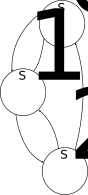
\includegraphics[width=0.98in]{arbiter_fsm.pdf}
    \caption{Arbiter FSM}
  \end{subfigure}
  \begin{subfigure}[b]{0.3\textwidth}
    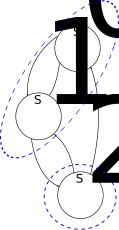
\includegraphics[width=1.3in]{arbiter_fsm_grouped.pdf}
    \caption{L-equivalence groupings }
  \end{subfigure}
  \begin{subfigure}[b]{0.3\textwidth}
    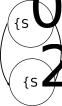
\includegraphics[width=0.69in]{drawing.pdf}
    \caption{L-equivalence digraph}
  \end{subfigure}
\end{figure}

Therefore, a reasonable approach is to view FSMs more abstractly than as group 
of assignments to register variables. Then, if all FSM traces produce the same 
$l$-projection, it satisfies noninterference. As an example, Figure 2a shows a 
pictorial representation of the FSM from the code segment in Listing 1. To 
consider only the state transitions that an attacker at level $l$ can observe, 
we begin by grouping together all the adjacent FSM states which are 
$l$-equivalent as in Figure 2b. In this case, the transitions between $S_0$ and 
$S_1$ can't be observed by the attacker, only the transitions between $S_0$ and 
$S_2$ can. Finally, we use these sets of FSM states to produce a new directed 
graph in Figure 2c. Since each node has at most a single outgoing edge, the 
$l$-projections of all traces through the FSM are equivalent.

This approach can be applied in general
by viewing an FSM as a directed graph $F=(S,E)$ where the nodes $s\in S$ are 
FSM states (not to be confused with states $\sigma$ which are mappings from 
variables to values) and edges are state transitions of the form $(s_1,s_2)$ 
indicating thatn $s_1$ can transition to $s_2$. (Note that in this model 
the conditions on which state transitions happen are ignored). 

We say that a state $s_1$ \emph{$l$-observably transitions to} a state $s_2$, 
written $s_1 \rightsquigarrow_l s_2$ if $s_2$ is the nearest state along the 
closure of state transitions from $s_1$ such that $s_1 \not\approx_l s_2$. Or 
more formally,
\begin{align*}
  s_1 \rightsquigarrow s_2 \Longleftrightarrow
    & s_1 \not\approx_l s_2 \wedge \\
    & ((s_1,s_2)\in E \\
    \vee & \left( (s_1,s)\in E \wedge s_1 \approx_l s\wedge s \rightsquigarrow s_2 \right)
    )
\end{align*}
where $s_1 \approx s_2$ if the states $\sigma_1$ and $\sigma_2$ for each of 
those FSM states are low equivalent.

\begin{figure}
\begin{align*}
FSM & ::= s_1,\ldots s_n \\
s & ::= (T_s, T_v) \\
T_s & ::= \mathtt{case}(e)[s_1, \ldots,s_n] \\
T_v & ::= x_1=e_1, \ldots, x_n=e_n
\end{align*}
\caption{A Finite State Machine Syntax}
\label{fig:fsm_syntax}
\end{figure}

\begin{figure}
\[
  \inferrule
    {
      s_i = (T_{si},T_{vi}) \\
      \vdash T_s : N, M
    }{
      \vdash (T_s, T_v) : \{s_i| s_i\in N \wedge
      T_{vi}\not\approx_l T_v
      \vee(T_{vj} \approx_l T_v \wedge s_i \in M(s_j))\}
    }
\]

\[
  \inferrule
  {
    \vdash s_i : L_i
  }{
    \mathtt{case}(e)[s_1,\ldots,s_n] :
    \{s_1,\ldots,s_n\},\{(s_1,L_1),\ldots,(s_n,L_n)\}
  }
\]

\[
  \inferrule
  {
    e_i \Downarrow v_i
  }{
    \vdash x_i=e_1,\ldots,x_n=e_n :
    \{(x_i,v_i),\ldots,(x_n,v_n)\}
  }
\]

\[
  \inferrule
  {
    \vdash T_{v1} : U_1 \\ \vdash T_{v2} : U_2 \\ 
    \forall x \in \{x_i|\Gamma(x_i)\sqsubseteq l\}.U_1(x)=U_2(x)
  }{
    T_{v1} \approx_l T_{v2}
  }
\]

\[
  \inferrule
  {
    \vdash T_{v1} : U_1 \\ \vdash T_{v2} : U_2 \\
    \exists x \in \{x_i|\Gamma(x_i)\sqsubseteq l\}.U_1(x)\neq U_2(x)
  }{
    T_{v1} \not\approx_l T_{v2}
  }
\]

\[
  \inferrule
  {
    s_i = (T_{si}, T_{vi}) \\
    \forall s_j,s_j \in \{s|s_i \rightsquigarrow_l s\}. T_{vj} \approx_l T_{vk}
  }{
    \vdash s_1,\ldots,s_n
  }
\]

\label{fig:types}
\caption{A Type System for Timing Insensitive Noninterference}
\end{figure}


Figure 3 shows a simplified syntax for describing finite state machines. An FSM
is a sequences of states $s$. States are pairs consiting of state transition
tables $T_s$ and output tables $T_v$. A state transition table is a single case
statement producing a next state. This guarantees that the next states are
mutually exclusive and the FSM is deterministic. Output tables are a sequence
of assignments to variables.

Figure 4 shows a type system that enforces timing insensitive noninterference.
The typing rule for states produces a set $L$ of the states that it can
$l$-observably transition to. State transition tables produce two sets. $N$ is
simply the set of states that can be transitioned to in the table and $M$ is a
mapping from the states in the table to the sets of states that each of them
can $l$-observably transition to. The rule for states produces $L$ by checking
if it is $l$-equivalent to each state in $N$. If it isn't, it inserts that state
into $L$, otherwise, it gets the $L$ set of that state from $M$.

The three rules for output tables are used for determining if two states are 
$l$-equivalent by producing a mapping from the variables it updates to the 
big-step values of the expressions they are assigned. Finally, the rule for 
FSMs checks that for each state, all of the states it can $l$-observably 
transition to are $l$-equivalent. In other words, all outgoing transitions from 
this state appear the same to the attacker.

One flaw of this approach is that it is unlikely complete with respect to the 
high-stutter-equivalent formulation of noninterference. Since it disregards the 
conditions on which state transitions happen, extra information that could be 
used to determine if an attacker visible transition could take place is lost. 
It is also unclear how and how well the values of expressions can be determined 
by the type system for the purpose of checking $l$-equivalence in the rule for 
output tables.

\end{document}
